\newpage 
\section{Вычисление несобственных интегралов с использование вычетов. Лемма Жордана и теорема о вычислении несобственного интеграла от рациональной функции с помощью вычетов.}

\textbf{Лемма Жордана:}\\[2mm]
Пусть  $f(z)$ --- непрерывная функция в $\{Im\,z \geq 0\}$ за исключением изолированного множества точек;

$\gamma_{R} =\{z\in\mathbb{C}: \, |z|=R, \, Im\,z\geq 0\}$;

$M(R)=\underset{z\in \gamma_{R}}{\max}|f(z)|, \, M(R) \rightarrow 0$ при $R\rightarrow \infty$;\\[2mm]
Тогда $\forall \lambda > 0 \, \int\limits_{\gamma_{R}} f(z)e^{i\lambda z}dz\rightarrow 0$\\[4mm]

\textbf{Теорема о вычислении несобственного интеграла от рациональной функции с помощью вычетов:}\\[2mm]
Пусть  $f(x)=\frac{P_m(x)}{Q_n(x)}$, где $P_m(x), Q_n(x)$ -- многочлены степени $m$ и $n$ соответственно, $n\geq m+2$;

$Q_n(x)\neq 0$ при $x \in \mathbb{R}$ (не имеет действительных корней);\\[2mm]
Тогда $\int\limits_{-\infty}^{+\infty}f(x)dx=2\pi i \sum_{j=1}^k res\,f(z_j)$, 

где $z_1, ...,z_k$ -- все полюса $f$ в области $Im\,z >0$

\begin{proof}
    \ \\
    \begin{figure}[h]
        \centering
        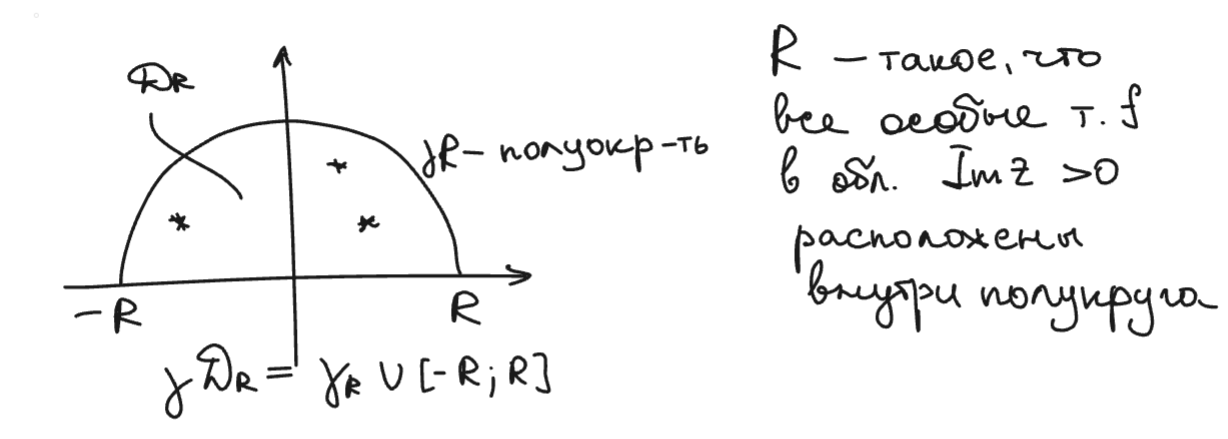
\includegraphics[width=1\linewidth]{answers/img/ans21.png}
    \end{figure}

    Так как $f$ непрерывна на компакте $\gamma_R$, то $\exists \underset{z\in \gamma_R}{\max} |f(z)|$.\\[2mm]
    $\max\frac{|P_m(z)|}{|Q_n(z)|}=\underset{|z|=R, Im\,z\geq0}{\max} \frac{|b_mz^m+...|}{|a_nz^n+...|} \sim{} \underset{|z|=R, Im\,z\geq0}{\max} \frac{|b_m||z|^m}{|a_n||z|^n}= $\\[2mm]
    $=\underset{|z|=R}{\max}\frac{|b_m|}{|a_n|}\cdot\frac{1}{|z|^{n-m}}\sim{} \frac{|b_m|}{|a_n|}\cdot \frac{1}{R^{n-m}}$\\[2mm]
    Пусть $L(\gamma_R)$ -- длина $\gamma_R$. Тогда:\\[2mm]
    $\left|\int\limits_{\gamma_R}f(z)dz\right|\leq \underset{a\in\gamma_R}{\max}|f(z)|\cdot L(\gamma_R)\sim c\frac{1}{R^{n-m}}\pi R = \frac{c\pi}{R^{n-m-1}}\to 0$ при $R\to \infty, n-m-1>0$\\[2mm]
    Откуда следует, что $\left|\int\limits_{\gamma_R} f(z)dz\right| \to 0$ при $R\to \infty$.\\[2mm]
    По теореме Коши: $\oint\limits_{\gamma D_R}f(z)dz = 2\pi i \sum\limits_{j=1}^k res\, f(z_j)$ не зависит от $R$, при $R\to \infty:$\\[2mm]
    $\oint\limits_{\gamma D_R}f(z)dz = \int\limits_{\gamma_R}f(z)dz + \int\limits_{-R}^R f(x)dx \to 0+\int\limits_{-\infty}^{-\infty}f(x)dx$.
\end{proof}


\newpage
\textbf{Пример вычисления несобственного интеграла от тригонометрических функций:}\\
Вычислить интеграл $\int\limits_{-\infty}^{+\infty} \frac{x\cos x dx}{x^2-2x+10}$\\
Функция $f(z)=\frac{ze^{iz}}{z^2-2z+10}$ удовлетворяет условиями леммы Жордана. Здесь $t=1$ и $F(z)=\frac{z}{z^2-2z+10}$. Особыми точками функции $f(z)$ являются полюсы первого порядка $z=1\pm 3i$. В верхней полуплоскости иммется единственная особая точка $z=1+3i$. Вычислим относительно этой точки вычет функции $f(z)$:
$$res\, f(1+3i) = \frac{ze^{iz}}{(z^2-2z+10)'}=\frac{(1+3i)e^{-3+i}}{6i}$$
Следовательно, $\int\limits_{-\infty}^{+\infty} \frac{xe^{ix}dx}{x^2-2x+10}=2\pi i \frac{(1+3i)e^{-3+i}}{6i} = \frac{\pi}{3}e^{-3}(1+3i)(\cos 1+i\sin 1)=\frac{\pi}{3} e^{-3}(\cos 1 - 3\sin 1)+i\frac{\pi}{3}e^{-3}(3\cos 1+\sin 1).$\\
Сравнивая в обеисх частях этого равенства действительные и мнимые части с учитывая, что $$\int\limits_{-\infty}^{+\infty}\frac{xe^{ix}dx}{x^2-2x+10}=\int\limits_{-\infty}^{+\infty}\frac{x\cos x\, dx}{x^2-2x+10}+i\int\limits_{-\infty}^{+\infty}\frac{x\sin x\, dx}{x^2-2x+10}$$ 
получим $$\int\limits_{-\infty}^{+\infty}\frac{x\cos x\, dx}{x^2-2x+10} = \frac{\pi}{3}e^{-3}(\cos 1-3\sin 1),$$
$$\int\limits_{-\infty}^{+\infty}\frac{x\sin x\, dx}{x^2-2x+10} = \frac{\pi}{3}e^{-3}(3\cos 1+\sin 1),$$
